\documentclass{beamer}
\setbeamertemplate{footline}[page number]
\date{}
\author{}
\institute{}

%%%%%%% Put these names back in the final version 
%\\Aswathy Rajendra Kurup\\Meenu Ajith}
%\institute{Department of Electrical and Computer Engineering\\The University of New Mexico}
\setbeamercovered{transparent}
\usepackage{setspace}
\usepackage{array}
\usepackage[T1]{fontenc}
\usepackage{graphicx}
\usepackage{amsmath}
\usepackage{amsfonts}
\usepackage{amssymb}
\usepackage{makeidx}
\usefonttheme{serif}
\usepackage{multirow}
\usepackage{booktabs} 
\usepackage{rotating}
\usepackage{color}
\usepackage{float}
\usepackage[latin1]{inputenc}
\usepackage[english]{babel}
\usepackage{amsmath}
\usepackage{amsfonts}
\usepackage{eurosym}
\usepackage{rotating}
\usepackage{multicol}
\usepackage{pythonhighlight}
\usepackage[normalem]{ulem}
\newcommand{\ba}{{\bf a}}
\newcommand{\bb}{{\bf b}}
\newcommand{\bc}{{\bf c}}
\newcommand{\bd}{{\bf d}}
\newcommand{\be}{{\bf e}}
\newcommand{\bbf}{{\bf f}}
\newcommand{\bg}{{\bf g}}
\newcommand{\bh}{{\bf h}}
\newcommand{\bi}{{\bf i}}
\newcommand{\bk}{{\bf k}}
\newcommand{\bl}{{\bf l}}
\newcommand{\bm}{{\bf m}}
\newcommand{\bn}{{\bf n}}
\newcommand{\bo}{{\bf o}}
\newcommand{\bp}{{\bf p}}
\newcommand{\bq}{{\bf q}}
\newcommand{\br}{{\bf r}}
\newcommand{\bs}{{\bf s}}
\newcommand{\bt}{{\bf t}}
\newcommand{\bu}{{\bf u}}
\newcommand{\bv}{{\bf v}}
\newcommand{\bw}{{\bf w}}
\newcommand{\bx}{{\bf x}}
\newcommand{\by}{{\bf y}}
\newcommand{\bz}{{\bf z}}

\newcommand{\bA}{{\bf A}}
\newcommand{\bB}{{\bf B}}
\newcommand{\bC}{{\bf C}}
\newcommand{\bE}{{\bf E}}
\newcommand{\bG}{{\bf G}}
\newcommand{\bH}{{\bf H}}
\newcommand{\bI}{{\bf I}}
\newcommand{\bK}{{\bf K}}
\newcommand{\bL}{{\bf L}}
\newcommand{\bM}{{\bf M}}
\newcommand{\bO}{{\bf O}}
\newcommand{\bQ}{{\bf Q}}
\newcommand{\bR}{{\bf R}}
\newcommand{\bS}{{\bf S}}
\newcommand{\bT}{{\bf T}}
\newcommand{\bV}{{\bf V}}
\newcommand{\bW}{{\bf W}}
\newcommand{\bX}{{\bf X}}
\newcommand{\bY}{{\bf Y}}
\newcommand{\bZ}{{\bf Z}}
\newcommand\uptocnt{\stackrel{\mathclap{\normalfont\mbox{c}}}{\propto}}
\newcommand{\bpt}{{\bf pt}}
\newcommand{\bpl}{{\bf pl}}
\newcommand{\bdp}{{\bf dp}}
\newcommand{\btemp}{{\bf temp}}

\newcommand{\bmu}{{\boldsymbol \mu}}
\newcommand{\bSigma}{{\boldsymbol \Sigma}}
\newcommand{\bsigma}{{\boldsymbol \sigma}}
\newcommand{\bvarPhi}{{\boldsymbol \varPhi}}
\newcommand{\bvarphi}{{\boldsymbol \varphi}}
\newcommand{\bPhi}{{\boldsymbol \Phi}}
\newcommand{\bdelta}{{\boldsymbol \delta}}
\newcommand{\bZero}{{\bf 0}}
\newcommand{\bOne}{{\bf 1}}
\newcommand{\balpha}{{\boldsymbol \alpha}}
\newcommand{\bAlpha}{{\boldsymbol A}}
\newcommand{\btheta}{{\boldsymbol \theta}}

\newcommand{\softmax}{\text{softmax}}
\newcommand{\diag}{\text{diag}}
\newcommand{\sinc}{\mathrm{sinc}}
\newcommand{\argmin}{\mathop{\mathrm{argmin}}}
\newcommand{\infl}{\eta}
\newcommand{\Ind}{\mathrm{I}}
\newcommand{\Real}{\mathbb R}
\newcommand{\Intg}{\mathbb Z}
\newcommand{\Complex}{\mathbb C}
\newcommand{\Natural}{\mathbb N}
\newcommand{\Fourier}[1]{\mathcal{F} \{#1\}}
%\newcommand{\ii}{\mathbbm{i}}
\newcommand{\bphi}{\boldsymbol{\mathit{\phi}}}

\newcommand{\hs}{\hspace{2pt}}
\newcommand{\sign}{\text{sign}}
\author{Manel Mart\'inez-Ram\'on\\Meenu Ajith\\Aswathy Rajendra Kurup}

\usetheme{Madrid}
\usecolortheme{beaver}
\usepackage{tikz}
\usetikzlibrary{fit,arrows,calc,positioning}
\usepackage{listings}
\usepackage{xcolor}
\usepackage{emerald} 
\usepackage[T1]{fontenc} 
\usepackage{verbatim}
\usepackage{graphicx}
\usepackage{epsfig}
\usepackage{psfrag}
\usepackage[english]{babel}
\usepackage{listings}
\usepackage{courier}
\usepackage{color}
 \usepackage{vwcol} 
 \usepackage[english]{babel} % To obtain English text with the blindtext package
\usepackage{blindtext}
\definecolor{codegreen}{rgb}{0,0.6,0}
\definecolor{codegray}{rgb}{0.5,0.5,0.5}
\definecolor{codepurple}{rgb}{0.58,0,0.82}
\definecolor{backcolour}{rgb}{0.95,0.95,0.92}

\lstdefinestyle{mystyle}{
  backgroundcolor=\color{backcolour},   commentstyle=\color{codegreen},
  keywordstyle=\color{magenta},
  numberstyle=\tiny\color{codegray},
  stringstyle=\color{codepurple},
  basicstyle=\ttfamily\footnotesize,
  breakatwhitespace=false,         
  breaklines=true,                 
  captionpos=b,                    
  keepspaces=true,                 
  numbers=left,                    
  numbersep=5pt,                  
  showspaces=false,                
  showstringspaces=false,
  showtabs=false,                  
  tabsize=2
}
\lstset{style=mystyle}

%% Stuff for movies

% %\newcommand{\bt}{{\bf t}}
% \newcommand{\br}{{\bf r}}
% \newcommand{\bs}{{\bf s}}
% \newcommand{\by}{{\bf y}}
% \newcommand{\bz}{{\bf z}}
% \newcommand{\bx}{{\bf x}}
% \newcommand{\bw}{{\bf w}}
% \newcommand{\be}{{\bf e}}
% \newcommand{\bbf}{{\bf f}}
% \newcommand{\bb}{{\bf b}}
% \newcommand{\bd}{{\bf d}}
% \newcommand{\bA}{{\bf A}}
% \newcommand{\bB}{{\bf B}}
% \newcommand{\bL}{{\bf L}}
% \newcommand{\bM}{{\bf M}}

% \newcommand{\bC}{{\bf C}}
% \newcommand{\bI}{{\bf I}}
% \newcommand{\bK}{{\bf K}}
% \newcommand{\bk}{{\bf k}}
% \newcommand{\bT}{{\bf T}}
% \newcommand{\bV}{{\bf V}}
% \newcommand{\bW}{{\bf W}}
% \newcommand{\bX}{{\bf X}}
% \newcommand{\bY}{{\bf Y}}
% \newcommand{\bZ}{{\bf Z}}
% \newcommand{\bm}{{\bf m}}
% \newcommand{\bpt}{{\bf pt}}
% \newcommand{\bpl}{{\bf pl}}
% \newcommand{\bdp}{{\bf dp}}
% \newcommand{\btemp}{{\bf temp}}
% \newcommand{\bl}{{\bf l}}
% \newcommand{\bu}{{\bf u}}
% \newcommand{\bmu}{{\boldsymbol \mu}}
% \newcommand{\bSigma}{{\boldsymbol \Sigma}}
% \newcommand{\bLambda}{{\boldsymbol \Lambda}}

% \newcommand{\bsigma}{{\boldsymbol \sigma}}
% \newcommand{\bvarphi}{{\boldsymbol \varPhi}}
% \newcommand{\btheta}{{\boldsymbol \theta}}
% \newcommand{\bZero}{{\bf 0}}
% \newcommand{\balpha}{{\boldsymbol \alpha}}
% \newcommand{\bpi}{{\boldsymbol \pi}}
% \newcommand{\bxi}{{\boldsymbol \xi}}
% \newcommand{\bdelta}{{\boldsymbol \delta}}
\lstset{
	language=Python,
	basicstyle=\footnotesize\ttfamily\color{black},
	commentstyle = \footnotesize\ttfamily\color{red},
	keywordstyle=\footnotesize\ttfamily\color{blue},
	stringstyle=\footnotesize\ttfamily\color{black},
%	columns=fixed,
%	numbers=left,    
	numberstyle=\tiny,
	stepnumber=1,
	numbersep=5pt,
	tabsize=1,
	extendedchars=true,
	breaklines=true,            
	frame=b,         
	showspaces=false,
	showtabs=true,
	xleftmargin=6pt,
	framexleftmargin=6pt,
	framexrightmargin=2pt,
	framexbottommargin=4pt,
	showstringspaces=false      
}

\lstloadlanguages{
         Python
}

%\graphicspath{ {./images/} }  % Figures path - used in graphicx

%\selectcolormodel{cmyk}

\mode<presentation>

\newcommand{\dred}{darkred!90!black}
\newcommand{\written}{\ECFJD\textcolor{cyan!50!white}}
\newcommand{\hlight}{\textcolor{\dred}}
\newcommand{\Ex}{\textcolor{\dred}{Ex. }}

% remove navigation symbols in full screen mode
\setbeamertemplate{navigation symbols}{}  
\setbeamertemplate{blocks}[rounded][shadow=false]
\setbeamercolor{note page}{fg=black}

\setbeamercolor{title}{fg=\dred}
\setbeamercolor{frametitle}{fg=white}
\setbeamercolor{frametitle}{bg=\dred}
\setbeamercolor{structure}{fg=black,bg=white}
\setbeamercolor{background canvas}{bg=white,fg=black}
\setbeamercolor{normal text}{fg=black,bg=white}
\setbeamercolor{item}{fg=red!80!black,bg=white!}
\addtobeamertemplate{block begin}{\setbeamercolor{block title}{fg=white,bg=\dred}
\setbeamercolor{block body}{fg=white,bg=gray}}{}


\title{5. Sequence modeling with recurrent neural networks}
\subtitle{5.6. Machine translation with encoder-decoder structures}

\addtobeamertemplate{frametitle}{}


\begin{document}
\maketitle

\begin{frame}{Introduction}
\begin{itemize}
    \item A translation machine consists of a deep structure whose inputs are sequences with variable lengths in a given \emph{input language} (e.g. English):
    \begin{center}
        \emph{Spring begins today.}
    \end{center}
 and whose outputs are sentences of a different length in a \emph{target language} (e.g. French): 
 \begin{center}
     \emph{Le printemps commence aujourd'hui.}
 \end{center}
\item Feedforward deep structures are limited in this task because both their inputs and outputs are of fixed length.
\item Recurrent structures have been used for this task.
\end{itemize}
\end{frame}

\begin{frame}{Introduction}
\begin{itemize}
    \item One of the first successful variable length machine translation schemes is given by Ilya Sutskever et al. (2014) while working at Google Inc.  
    \item The machine was constructed by a pair of input (encoder) LSTM and output (decoder) LSTM.
    \item The input uses a word embedding technique to code the words in vectors. 
    \item The word embedding matrix consists of a matrix of dimensions $D_d \times D_c$ corresponding to the number of words and the dimension of the embedding vector. 
    \item This is, each word in a dictionary for each language is encoded in a fixed length vector. 
\end{itemize}
    
\end{frame}

\begin{frame}{Structure}
\begin{center}
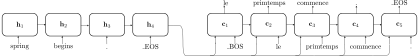
\includegraphics[scale=0.28]{Module 5 (RNN)/pics/sequence_translate_RNN.pdf}
\end{center}
\begin{itemize}
\item The first word \emph{spring} is entered, which generates state $\bh_1$, which is fed back  with the second word, to generate the next state. The operation is repeated to the \_EOS token. 
\item State $\bh_4$ is a fixed length code of the sentence. 
\item This state is used in another RNN. 
\end{itemize}
\end{frame}


\begin{frame}{Structure}
\begin{center}
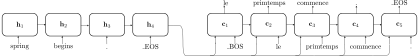
\includegraphics[scale=0.28]{Module 5 (RNN)/pics/sequence_translate_RNN.pdf}
\end{center}

\begin{itemize}
\item The output state $\bh_4$ is used as input of the next RNN, concatenated with a \_BOS token. 
\item This produces state $\bc_1$. This is used to decode the first word \emph{le}.
\item State $\bc_1$ is fed back together with $\bh_4$ and the first decoded word to produce state $\bc_2$, which is used to produce the second word. 
\item When the state is decoded as \_EOS, the translation is finished. 
\end{itemize}
\end{frame}


\begin{frame}{Structure}

\begin{itemize}
\item Usually, for the encoding and decoding sections, LSTM or GRU units are used. 
\item The words in the target language (French here) are obtained after the transformation of the hidden states $\bc_t$ of the decoder RNN through a dense neural network. 
\item The number of outputs of the NN corresponds to the number of words in the target dictionary.
\item The dense NN output estimates the probability of each word in the dictionary.
\item Criterion: Minimize the correct translation negative log-likelihood (NLL)
    \begin{equation}
        J_{ML} = -\frac{1}{|S|} \sum_{T,S} \log p\left(T|S\right)
    \end{equation}
    where $|\cdot|$ denotes the cardinality of $s$.
\end{itemize}
\end{frame}


\begin{frame}{Greedy search versus beam search}
Assume a dictionary with only four words:  A, B, C, and \_EOS.
\begin{itemize}
    \item An encoder-decoder system outputs 4 words in 4 consecutive steps. In the first step, the most probable word is A.
    \item When this word is fed back, the most probable word is B. The next most probable words are C and \_EOS.
    \item The sequence is illustrated in the table:
\end{itemize}
\begin{table}[]
    \centering
    \begin{tabular}{c||c|c|c|c|}
       & 1 & 2 & 3 & 4  \\
     \hline
     \hline
      A   & \textbf{0.5} & 0.1 & 0.1 & 0.0  \\   
     \hline
     B    & 0.3 & \textbf{0.4} & 0.2 & 0.1 \\   
     \hline
     C    & 0.2 & 0.3 & \textbf{0.4} & 0.3 \\   
     \hline
     \_EOS    & 0.0 & 0.2 & 0.3 & \textbf{0.6} \\  
     \hline
    \end{tabular}
\end{table}
\end{frame}
\begin{frame}{Greedy search versus beam search}
    \begin{itemize}
   
        \item A greedy search would output the sequence ``A'', ``B'', ``C'', \_EOS 
\begin{center}
This gives a probability $p(T|S) = 0.5 \cdot 0.4 \cdot 0.4 \cdot 0.6 = 0.048$.
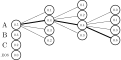
\includegraphics[scale=0.5]{Module 5 (RNN)/pics/greedy_search.pdf}
\end{center}
        \item A beam search uses  the $k$ words with the highest probability as input for the next steps.
        \item This changes the probabilities in the next steps
    \end{itemize}
\end{frame}

\begin{frame}{Beam search}
\vspace{-1cm}
\begin{multicols}{2}

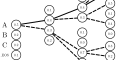
\includegraphics[scale=0.5]{Module 5 (RNN)/pics/beam_search.pdf}

\columnbreak

\begin{itemize}
\item With a beam $k=2$, the probabilities are
\end{itemize}
\begin{table}
    \centering
    \begin{tabular}{r|r}
 Path   Probability & NLL\\
 \hline
         $p$(ABCC|S) = 0.024 &0.4 \\
         $p$(ABC\_EOS|S) =  0.048 &\textbf{0.43}\\
         $p$(AB\_EOS|S) =   0.060 &\sout{0.61}\\
         $p$(ACCA) =   0.084 &0.01\\
         $p$(ACCB|S) = 0,021& 0.41\\
         $p$(AC\_EOS) =  0.030& \sout{0.76}\\
    \end{tabular}
\end{table}
\end{multicols}
The bold one is the finished sequence with the lowest NLL. The unfinished ones have lower NLL, so the search on their paths must be continued. The rest of the paths are discarded.
\end{frame}

\begin{frame}{Experiment}
 Sutskever et al describe the experimental setup as follows: 
\begin{itemize}
    \item Dataset: WMT 14 dataset, with 12 million sentences, 284 million French words, and 304 million English words.
    \item Dictionary: 160.000 English words (source) and 80.000 French words (target).
    \item Out-of-dictionary words were changed by a UNK (unknown) token.  
\item Translations produced by beam search. 
\item Source sentences reversed.
\end{itemize}
\end{frame}




\begin{frame}{Experiment}
\begin{itemize}
    \item Deep LSTMs with 4 layers of 1000 cells.
    \item 1000 dimension word embeddings.
    \item Softmax output over 80.000 words (without specification of the structure of the dense layers.)
    \item LSTM parameters initialized uniformly between -0.08 and 0.08.
    \item Momentum gradient descent with $\mu=0.7$. 7.5 epochs.
    \item Batches of 128 sequences. 
    \item Hard constraint on the norm of the weights. 
\end{itemize}
\end{frame}
\begin{frame}{Results}
\begin{itemize}
    \item Evaluation metric: Bilingual Evaluation Understudy. It is a number between 0 and 100 that compares automatic translations to high-quality reference translations. 

\begin{table}[]
    \centering
    \begin{tabular}{|l|l|}
\hline
\textbf{BLEU Score$^*$} & \textbf{Interpretation}\\
\hline
< 10 &	Almost useless\\
\hline
10 - 19 &	Hard to get the gist\\
\hline
20 - 29	& Clear gist, significant grammatical errors\\
\hline
30 - 40 &	Understandable to good translations\\
\hline
40 - 50	& High quality translations\\
\hline
50 - 60 &	Very high quality, adequate, fluent translations\\
\hline
> 60 &	Quality often better than human \\
\hline
\end{tabular}
\end{table}
    \footnotesize{$*$ See https://cloud.google.com/translate/automl/docs/evaluate. \\Google's  current BLEU for French as a target is higher tan 90.\\}
\end{itemize}
    
\end{frame}
\begin{frame}{Results}
\begin{table}[]
    \centering
    \begin{tabular}{|l|c|}
    \hline
       \textbf{Method} & \textbf{Test BLEU Score}\\
       \hline
       Bahdanau et al. [1] & 28.45\\
       \hline
       Baseline System [2] & 33.30\\
       \hline
       Single forward LSTM, beam size 12 & 26.17\\
       \hline
       Single reversed LSTM, beam size 12 & 30.59\\
       \hline
       Ensemble of 5 reversed LSTMs, beam size 1 & 33.00\\
       \hline
       Ensemble of 2 reversed LSTMs, beam size 12 & 33.27\\
       \hline
       Ensemble of 5 reversed LSTMs, beam size 2 & 34.50\\
       \hline
       Ensemble of 5 reversed LSTMs, beam size 12 & 34.81\\
       \hline
    \end{tabular}
\end{table}  


\footnotesize{1. D. Bahdanau, K. Cho, and Y. Bengio. Neural machine translation by jointly learning to align and translate.arXiv preprint arXiv:1409.0473, 2014\\
2.  H.  Schwenk.   Universit\'e  Le Mans.}



\end{frame}

\end{document}